\chapter{Dostupné datasety}
\label{sec:Datasets}
Před použitím konvoluční neuronové neuronové sítě navržené v této práci je nutné, aby byly váhy jednotlivých konvolucí správně nastaveny.
K tomuto účelu slouží tzv. trénovací množina.
Jedná se o množinu příkladů situací, na které může neuronová síť při svém fungování narazit.
V tomto případě, jelikož cílem sítě je určit počet lidí ve videosekvenci, se jedná o obrazy, resp. sekvenci po sobě jdoucích snímků.
Kromě samotných snímků potřebuje ještě síť základní pravdu, což je informace, pomocí které dokáže určit, jak moc se při svých predikcích mýlí, aby na základě této chyby mohla přenastavit své váhy, čímž tuto chybu sníží a posune se blíže optimu.
Tento typ strojového učení, kdy je pro natrénování modelu použita oanotovaná trénovací sada, se nazývá učení s učitelem.

Jelikož při samotném používání neuronové sítě již nedochází k žádnému přenastavování jejích vah, je pro zajištění jejího dobrého fungování naprosto stěžejní, aby byla trénovací množina rozsáhlá a co nejvíce různorodá.
Pokud je například síť natrénovaná pouze na snímcích získaných během dne, tak není zaručeno, že síť bude dosahovat stejně dobrých výsledků i na nočních záběrech.
Stejně tak model, natrénovaný na záběrech z bezpečnostních kamer, které jsou většinou umístěny vysoko nad lidskými hlavami, může mít problémy se záběry lidí pořízenými kamerou ve výšce očí.

Jelikož počítání lidí v obraze je mezi výzkumníky celkem populární problém, existuje k němu celá řada obsáhlých datasetů, z nichž některé jsou blíže popsány v této kapitole.
Mezi jednotlivými datasety ale mohou být veliké rozdíly a to nejen v rozlišení obsažených snímků, nebo velikosti davů, které snímky obsahují.
Rozdíly mohou být i v tom, jak jsou jednotlivé snímky anotovány, nebo v technologiích použítých pro pořízení těchto snímků.
To může být způsobeno například tím, kde má být daný estimátor nasazen, což bude určovat, jaké typy snímků bude dataset obsahovat.
Například datasety VisDrone \cite{VisDrone-Dataset-1, VisDrone-Dataset-2}, slouží k učení detekce, sledování a počítání objektů a lidí v obrazech a videích pořízených z dronu letícího desítky metrů nad zemí.
Oproti tomu snímky datasetu ShanghaiTechRGBD \cite{ShanghaiTechRGBD-1, ShanghaiTechRGBD-2} byly pořízeny ve zhruba dvoumetrové výšce pomocí RGB-D senzoru, což znamená, že kromě barevné složky snímky obsahují i hloubkovou informaci říkající, jak daleko od kamery se jednotlivé objekty ve scéně nacházejí.

\section{UCF-QNRF}
\begin{figure}[h!]
	\centering
	\subfloat[]{\includegraphics[height=3.5cm]{Figures/datasets/UCF-QNRF/img_0184.jpg}}
	\subfloat[]{\includegraphics[height=3.5cm]{Figures/datasets/UCF-QNRF/img_0222.jpg}}
	\subfloat[]{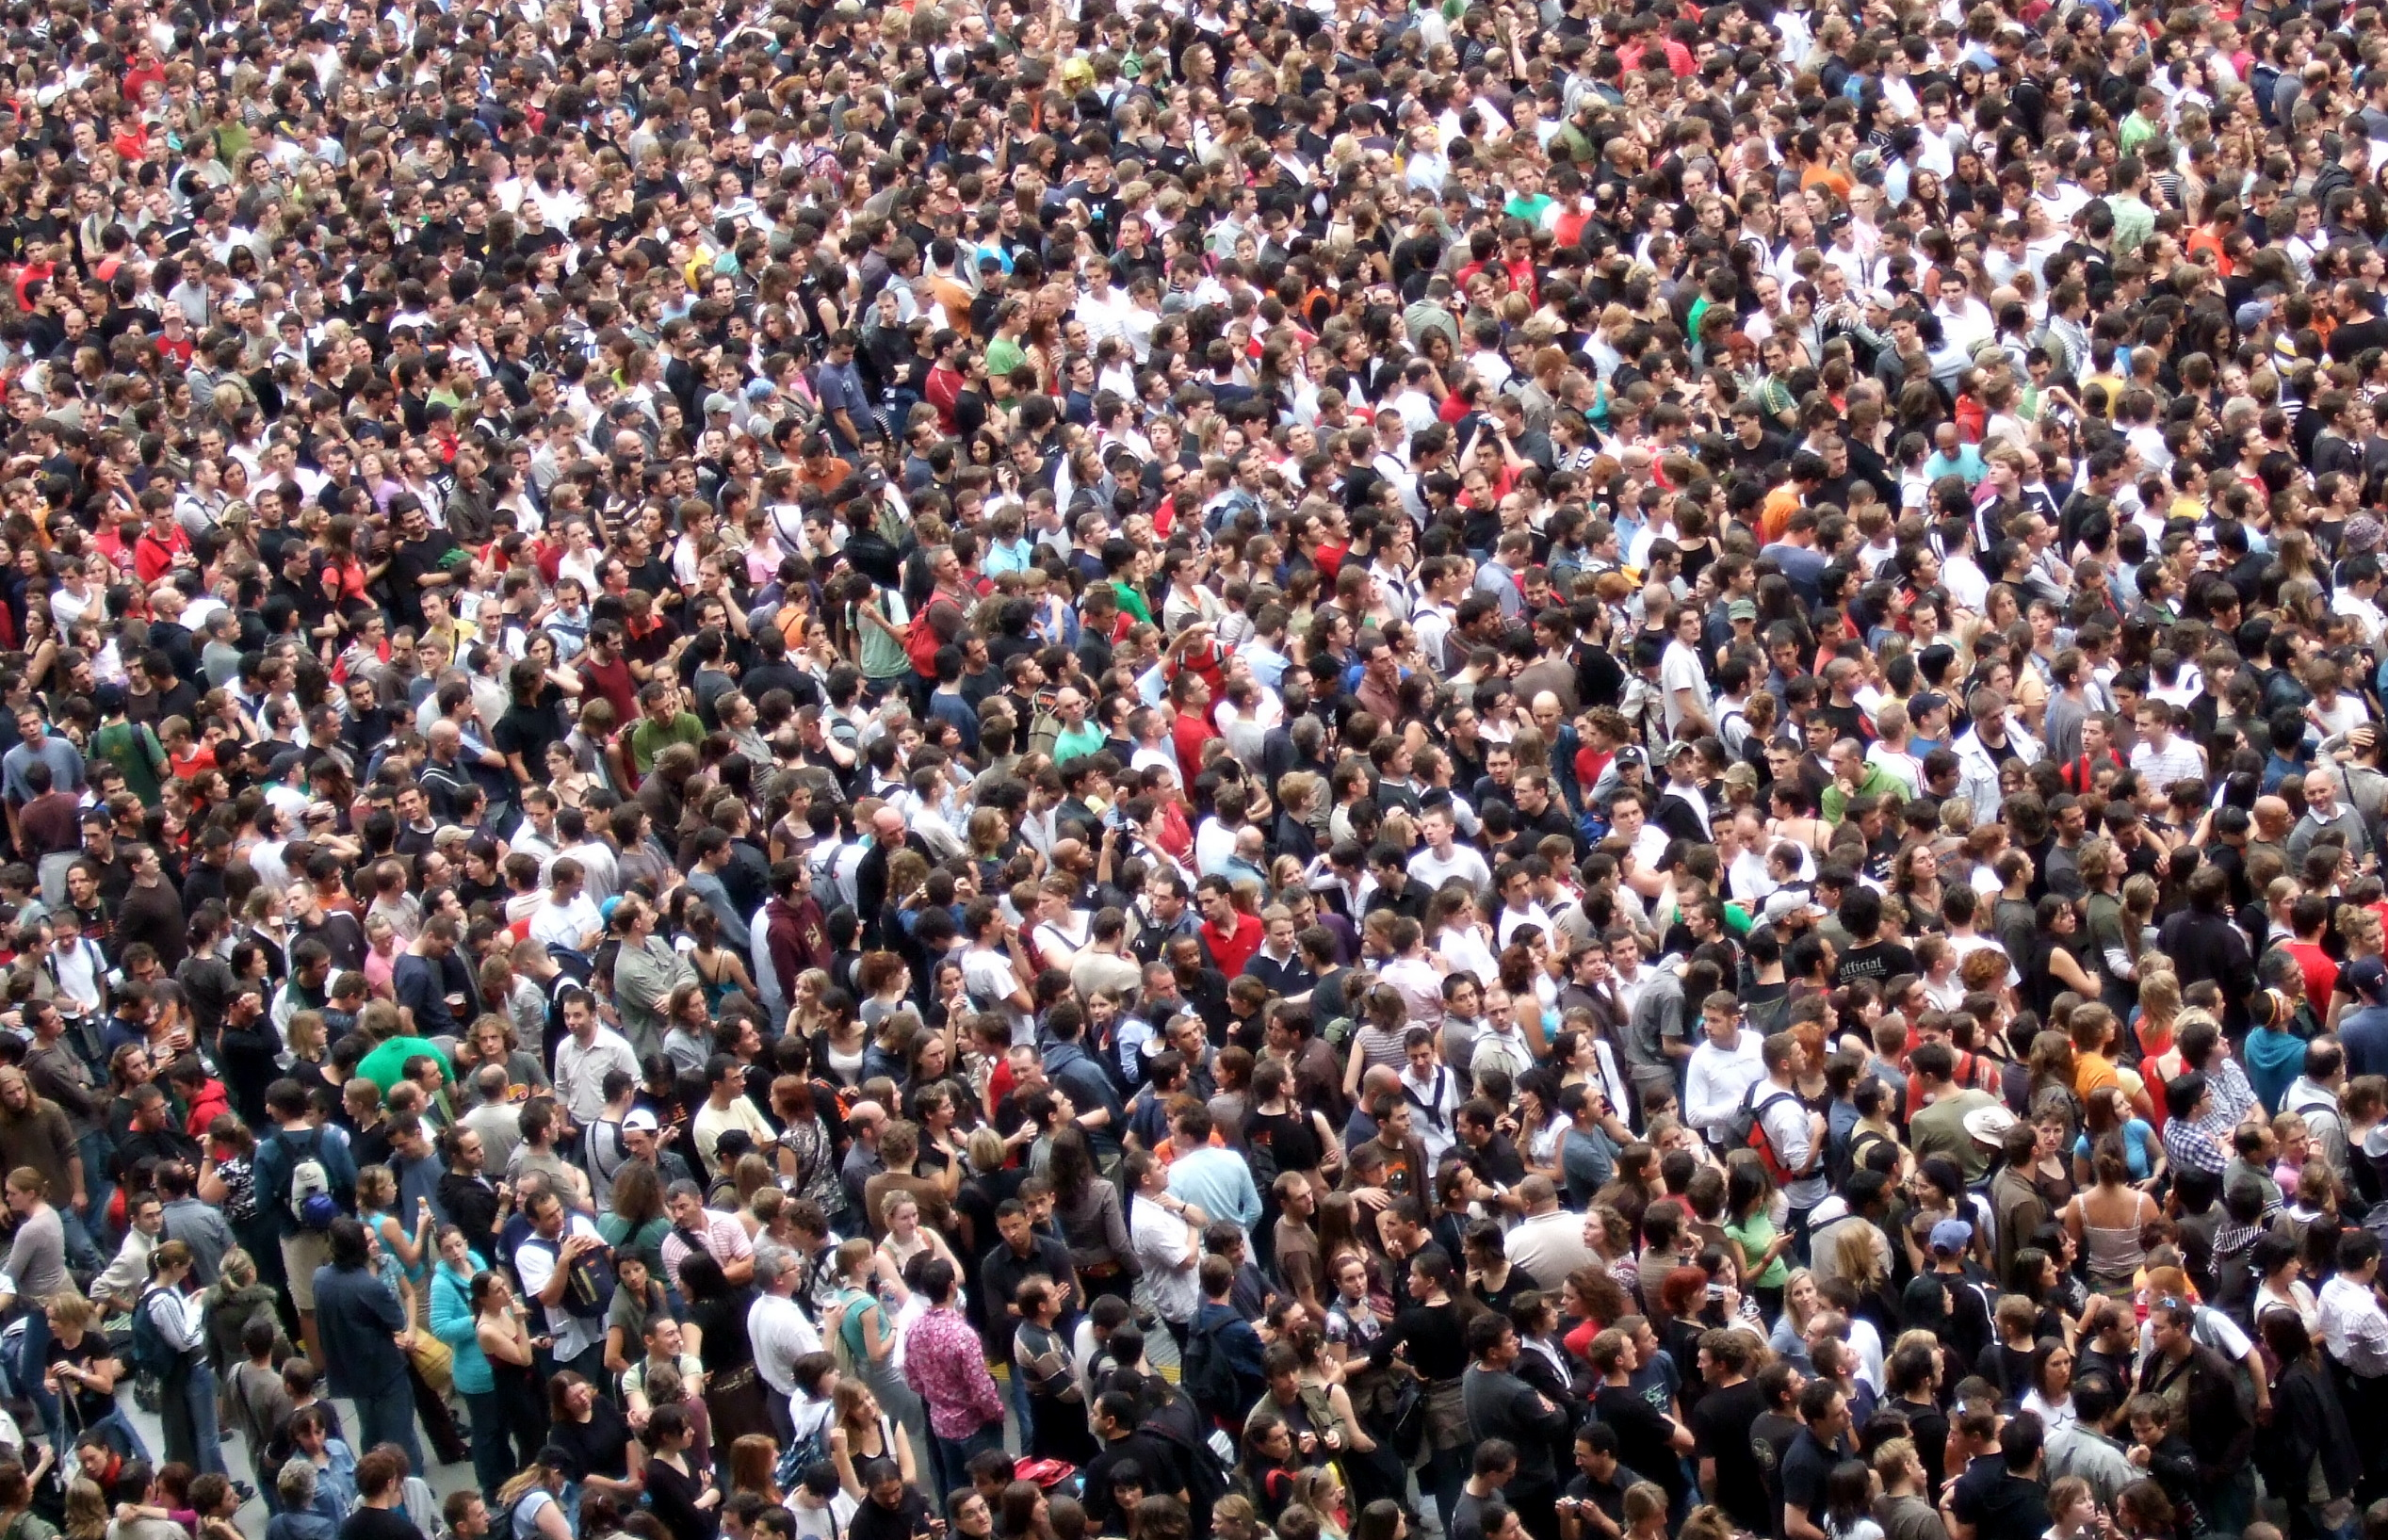
\includegraphics[height=3.5cm]{Figures/datasets/UCF-QNRF/img_0330.jpg}}
	\caption{Ukázka snímků obsažených v datasetu UCF-QNRF \cite{QNRF}}
	\label{fig:RNN_architecture}
\end{figure}

Dataset QNRF \cite{QNRF} z Kalifornské univerzity je jedním z nejpopulárnějších datasetů používaných pro trénování a validaci metod strojového učení počítajících lidi v obraze.
Je totiž jedním z nejrozsáhlejších datasetů, které jsou v současnosti volně dostupné.
Celkem obsahuje 1535 na sobě nezávislých snímků získaných z internetu.
Tyto snímky jsou rozděleny na trénovací množinu obsahující 1201 snímků a testovací množinu s 334 snímky.
Populární je nejen díky své velikosti, ale také kvůli tomu, že obsahuje velkou řadu velmi hustě zalidněných scén, což ukazuje průměrný počet lidí na jednotlivých snímcích tohoto datasetu, který se rovná 815 lidí na jeden obraz.
Všechny osoby jsou ve snímcích anotovány pomocí bodů, které se nachází v pozicích odpovídajícím středům jejich hlav.
Jeho další velkou výhodou je, že fotografie v něm obsažené jsou ve vysokém rozlišení.
Průměrná velikost těchto obrazů je 5,84 megapixelů.
Augmentací dat pomocí náhodného ořezávání jde proto snadno dataset rozšířit a získat tak mnohem větší trénovací množinu, která stále obsahuje snímky v dobré obrazové kvalitě.


\section{ShanghaiTech}
Dataset ShanghaiTech \cite{ShanghaiTech} je další z v této oblasti často používaných datasetů.
Jedná se o 1198 obrázků celkem obsahujících 330 165 osob, které jsou rozděleny do dvou částí.
V části ShanghaiTech Part-A je obsaženo 482 obrázků získaných z internetu, zatímco v ShanghaiTech Part-B se nachází 716 obrázků pořízených hustě zalidněných ulicích města Shanghai. Obě části jsou dále rozděleny na testovací a trénovací množiny.
Oproti UCF-QNRF nejsou snímky tohoto datasetu uložené v tak vysokém rozlišení. Průměrné rozlišení snímků první části je 0.5 megapixelů a druhé části 0.8 megapixelů.
Průměrný počet lidí je však i zde velmi vysoký, jelikož i v tomto datasetu řada snímků zachycuje velmi husté davy lidí. V první části se na snímku nachází v průměru 501 osob a v druhé části 124 osob.
Stjeně jako v UCF-QNRF je i zde každá osoba označena pouze jediným bodem, který je umístěný v pozici středu její hlavy.

\begin{figure}[h!]
	\centering
	\subfloat[]{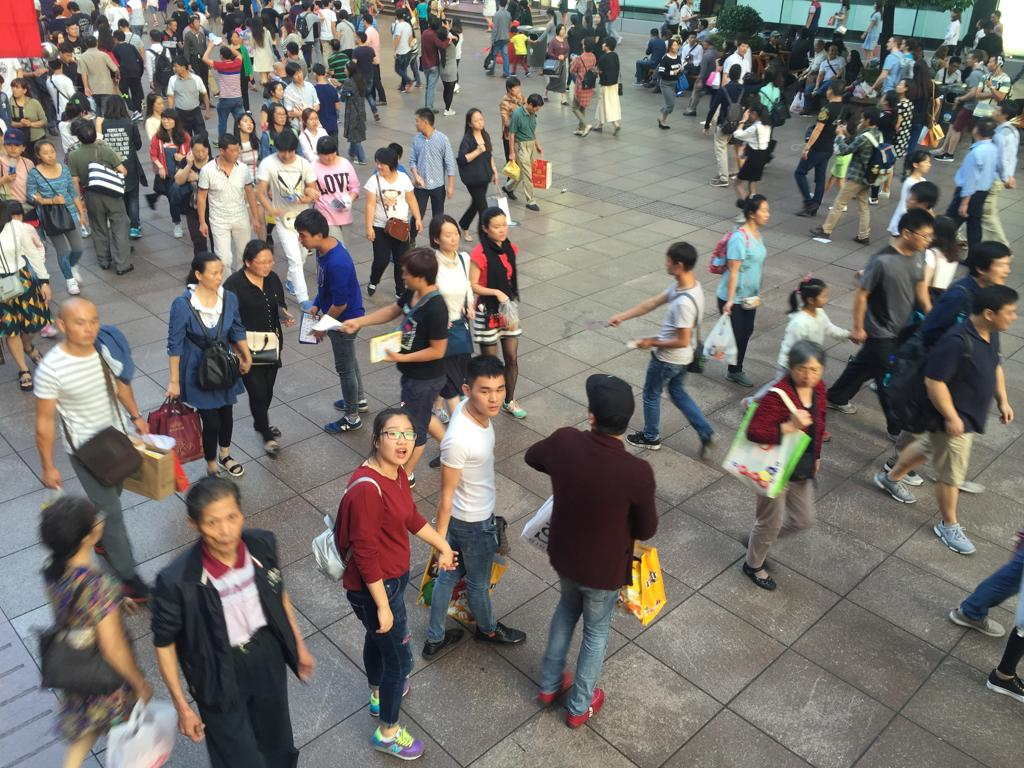
\includegraphics[height=3.5cm]{Figures/datasets/ShanghaiTech/IMG_21.jpg}}
	\subfloat[]{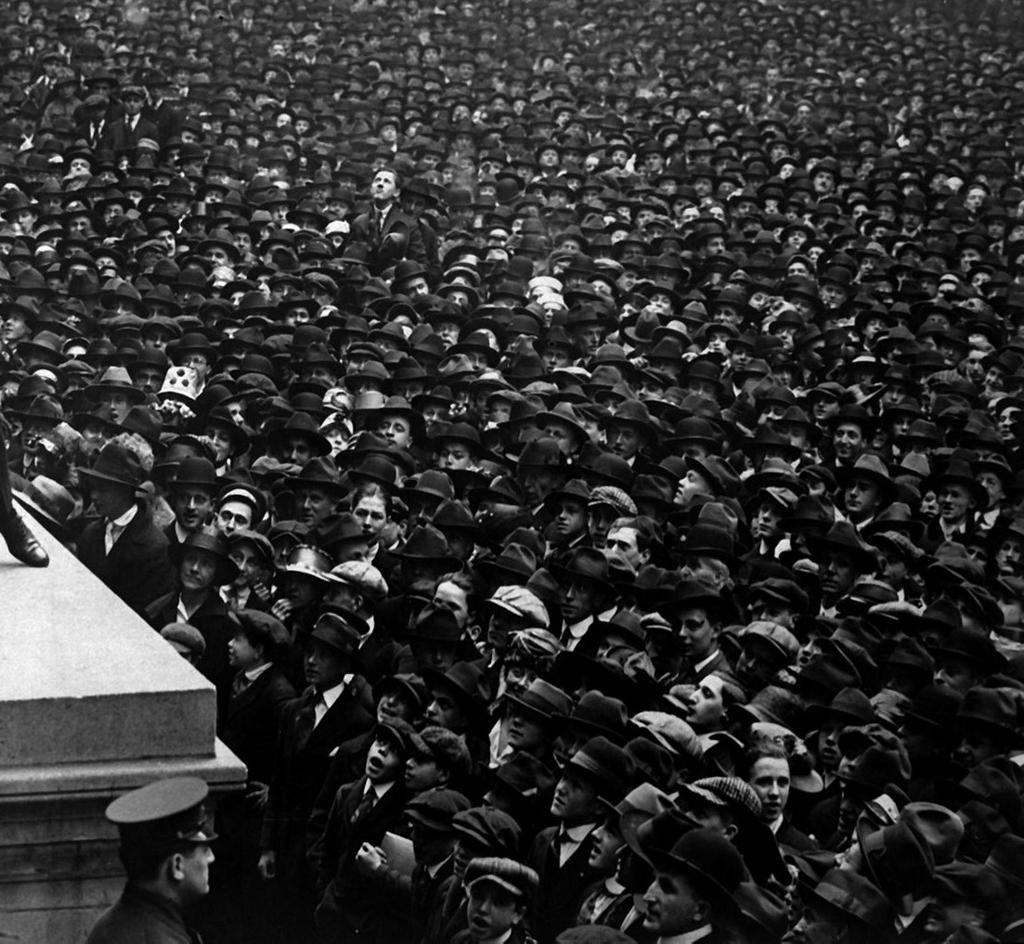
\includegraphics[height=3.5cm]{Figures/datasets/ShanghaiTech/IMG_168.jpg}}
	\subfloat[]{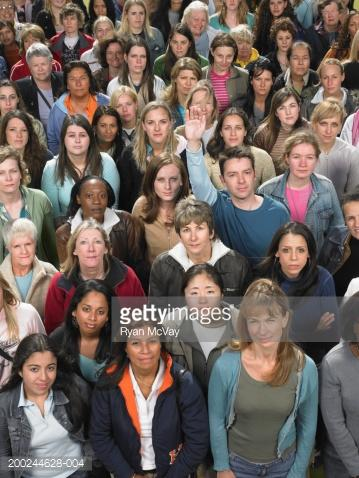
\includegraphics[height=3.5cm]{Figures/datasets/ShanghaiTech/IMG_272.jpg}}
	\subfloat[]{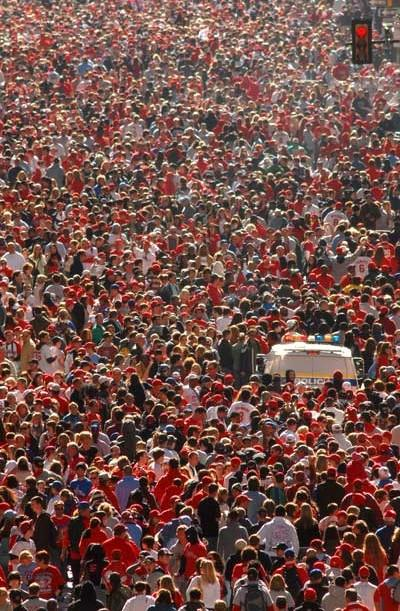
\includegraphics[height=3.5cm]{Figures/datasets/ShanghaiTech/IMG_115.jpg}}
	\caption{Ukázka snímků obsažených v datasetu ShanghaiTech \cite{ShanghaiTech}}
	\label{fig:RNN_architecture}
\end{figure}


\section{Fudan-ShanghaiTech}

\begin{table}[]
\begin{tabular}{|l|l|l|l|}
\hline
                    & \begin{tabular}[c]{@{}l@{}}počet\\ snímků\end{tabular} & \begin{tabular}[c]{@{}l@{}}průměrný počet\\ lidí na snímku\end{tabular} & \begin{tabular}[c]{@{}l@{}}průměrné\\ rozlišení snímku {[}px{]}\end{tabular} \\ \hline
UCF-QNRF            & 1535                                                   & 815                                                                     & 2013 * 2902                                                                  \\ \hline
ShanghaiTech Part-A & 482                                                    & 501                                                                     & 589 * 868                                                                    \\ \hline
ShanghaiTech Part-B & 716                                                    & 124                                                                     & 768 * 1024                                                                   \\ \hline
Fudan-ShanghaiTech  & 15 000                                                 & 26                                                                      & 1080 * 1920                                                                  \\ \hline
\end{tabular}
\end{table}


\endinput